
\documentclass[a4paper, 10pt, conference]{ieeeconf}

\IEEEoverridecommandlockouts
\overrideIEEEmargins

\usepackage{cite}
\usepackage{amsmath,amssymb,amsfonts}
\usepackage{graphicx}
\usepackage{color,calc}
\usepackage{makecell}
\usepackage{booktabs}
\usepackage{array}
\usepackage{ragged2e}
\usepackage{caption}
\usepackage{multirow}
\usepackage{url}
\captionsetup[lstlisting]{justification=raggedright, singlelinecheck=false}
\captionsetup{font=footnotesize}
\usepackage{listings}
\usepackage{xcolor}
\usepackage{tabularx}
\usepackage{pifont}
\usepackage{subcaption}
\usepackage{fancyhdr}
\newcommand{\cmark}{\ding{51}}
\newcommand{\xmark}{\ding{55}}

\def\BibTeX{{\rm B\kern-.05em{\sc i\kern-.025em b}\kern-.08em
    T\kern-.1667em\lower.7ex\hbox{E}\kern-.125emX}}

\lstset{
  basicstyle=\ttfamily\scriptsize,
  columns=fullflexible,
  keepspaces=true,
  breaklines=true,
  frame=single,
  framesep=2pt,
  xleftmargin=2pt,
  xrightmargin=2pt,
  aboveskip=2pt,
  belowskip=2pt,
}
\fancypagestyle{arxiv}{%
  \fancyhf{}
  \renewcommand{\headrulewidth}{0pt}
  \chead{\footnotesize Presented at the Robot Meets Prior Maps Workshop, ICRA 2026}
}

\title{\LARGE \bf RoboBIM: Scaling Robot Semantic Foundations through Agentic Extraction of BIM Priors}
\author{
\IEEEauthorblockN{Ashwin Nedungadi\IEEEauthorrefmark{*}, Bharathi Kannan Nithyanantham\IEEEauthorrefmark{*}, and Stefan Luedtke\thanks{\textsuperscript{*}Equal Contribution.}}\\
\IEEEauthorblockA{\textit{Institute for Visual \& Analytical Computing, Universit\"at Rostock} \\
\{ashwin.nedungadi, bharathikannan.nithyanantham, stefan.luedtke\}@uni-rostock.de}
}
%
\begin{document}
%
\maketitle
\thispagestyle{arxiv} % Replaces \thispagestyle{empty}
\pagestyle{empty}
% \thispagestyle{empty}
% \pagestyle{empty}

% ================================================================
% ABSTRACT
% ================================================================
\begin{abstract}
Building Information Models (BIM) stored in the Industry Foundation Classes (IFC) format contain rich priors for indoor robot autonomy. However, most pipelines use static one-pass conversions that produce occupancy maps or simulation assets while leaving much of the semantic information unused. We present RoboBIM, an agentic pipeline that converts IFC files into metric-semantic navigation contracts. RoboBIM separates structural extraction from semantic enrichment. First, a deterministic backbone creates a reliable geometric baseline, including occupancy maps, waypoints, and room topology. Then, an LLM agent infers missing semantic information, such as room types, hazards, and traversability, through sandboxed code execution. We also introduce an online query agent that retrieves these priors during robot operation. We evaluate RoboBIM on four public IFC models. The results show that RoboBIM helps close the semantic gap by increasing room-type coverage by about 74.5\% and filling previously empty semantic fields. The enriched graph natively exports to ROS~2 formats and natural-language summaries to ground scalable autonomy.
\end{abstract}

% ================================================================
% I. INTRODUCTION
% ================================================================
\section{Introduction}

Mobile robots deployed in structured indoor environments often build metric-semantic maps using onboard perception pipelines, such as Kimera~\cite{rosinol2021kimera} and Hydra~\cite{hughes2024hydra}, even when high-fidelity digital twins already exist as design-time Industry Foundation Classes (IFC) models~\cite{hamieh2021, follini2020, kim2022semantic}. This repeated mapping process ignores valuable architectural priors and forces the robot to spend time rediscovering known structures. However, raw IFC files cannot be used directly as navigation maps. IFC is the standard data schema for building models, but its semantic information is often incomplete or not organized for robotic use. Although IFC models can provide precise geometry, they often lack the functional information needed for safe autonomy. For example, room functions may be missing, and floor material properties may be attached to structural elements, such as floor slabs, rather than to the navigable spaces themselves. Since these attributes are often omitted or distributed across different levels of the IFC hierarchy, deterministic parsers struggle to extract a unified, robot-ready prior.

\textbf{The IFC semantic gap.} Existing IFC-to-graph pipelines usually follow a fixed process: they extract \texttt{IfcSpace} entities, segment space with a generalized Voronoi diagram (GVD), add door waypoints, and export the result to ROS~2 formats~\cite{teo2018igit, lin2020igssnn, zhu2024graph, ifcgraph2025, constructionrobotics2023}. These pipelines can reliably produce occupancy grids, room-transition graphs, and waypoint maps. However, their semantic output is limited by the information that is explicitly available in the IFC schema.

% \textbf{Monolithic LLM consumption is unsafe.} A possible alternative is to give the raw IFC file to a frontier LLM and ask it to produce a robot briefing. Prior work shows that LLMs can reason over BIM in principle, including MCP4IFC~\cite{nithyanantham2025mcp4ifc}, ifcMCP~\cite{lin2025ifcmcp}, modular MCP-BIM architectures~\cite{mcpbimarch2025}, Text2BIM~\cite{du2024text2bim}, and BIM2RDT~\cite{bim2rdt2025}. However, these systems can tolerate ambiguity in ways that robot navigation priors cannot. A hallucinated corridor, a fabricated door width, or a missing storey can corrupt downstream planning and may be hard to detect during runtime. Existing LLM-based BIM pipelines do not guarantee that LLM-enriched outputs preserve the deterministic topological baseline.

\textbf{Our contribution.} RoboBIM addresses this gap with a deterministic backbone and a staged LLM layer. The backbone first extracts the structural graph $\mathcal{G}_{\text{static}}=(\mathcal{O},\mathcal{W},\mathcal{T})$. Then, a seven-stage agentic layer enriches this graph with semantic fields that the deterministic backbone cannot infer. The pipeline produces a versioned navigation contract that integrates occupancy maps, waypoint graphs, topology, semantic annotations, and per-field confidence scores.

% \textbf{Monolithic LLM consumption is unsafe.} A tempting alternative is to submit the raw IFC to a frontier LLM and request a robot briefing. Prior works demonstrate that LLMs can reason over BIM in principle MCP4IFC~\cite{nithyanantham2025mcp4ifc}, ifcMCP~\cite{lin2025ifcmcp}, modular MCP-BIM architectures~\cite{mcpbimarch2025}, Text2BIM~\cite{du2024text2bim}, and BIM2RDT~\cite{bim2rdt2025}. However these systems are tolerant of ambiguity in ways that robot priors are not. A hallucinated corridor, a fabricated door width, or a silently dropped storey can corrupt downstream planning under failure modes that are difficult to detect at runtime. None of these pipelines provide a mechanism that guarantees the LLM-augmented output never degrades the deterministic topological baseline.

Fig.~\ref{fig:system_architecture} shows the full RoboBIM vision. The top part shows the offline agentic IFC-to-prior compiler. The bottom part shows a future online dual-agent navigation loop. This paper focuses on the offline compiler. The online loop is discussed briefly in Sec.~\ref{sec:outlook} and left for future work.

Concretely, we make the following contributions:
\begin{enumerate}
\setlength{\itemsep}{1pt}
\item We introduce a three-layer navigation graph extracted from IFC in a top-down manner. The graph is designed for robot use and can be exported directly to Nav2, Open-RMF, GraphML, and GeoJSON.

\item We propose a staged LLM agent that tunes backbone hyperparameters within fixed ranges, infers missing semantic fields, and produces a deterministic natural-language briefing for an onboard robot LLM.

\item We provide a preliminary evaluation on four public IFC models. RoboBIM increases room-type coverage, fills hazard, material, traversability, and policy fields that are null in the baseline.
\end{enumerate}


\begin{figure*}[t]
\centering
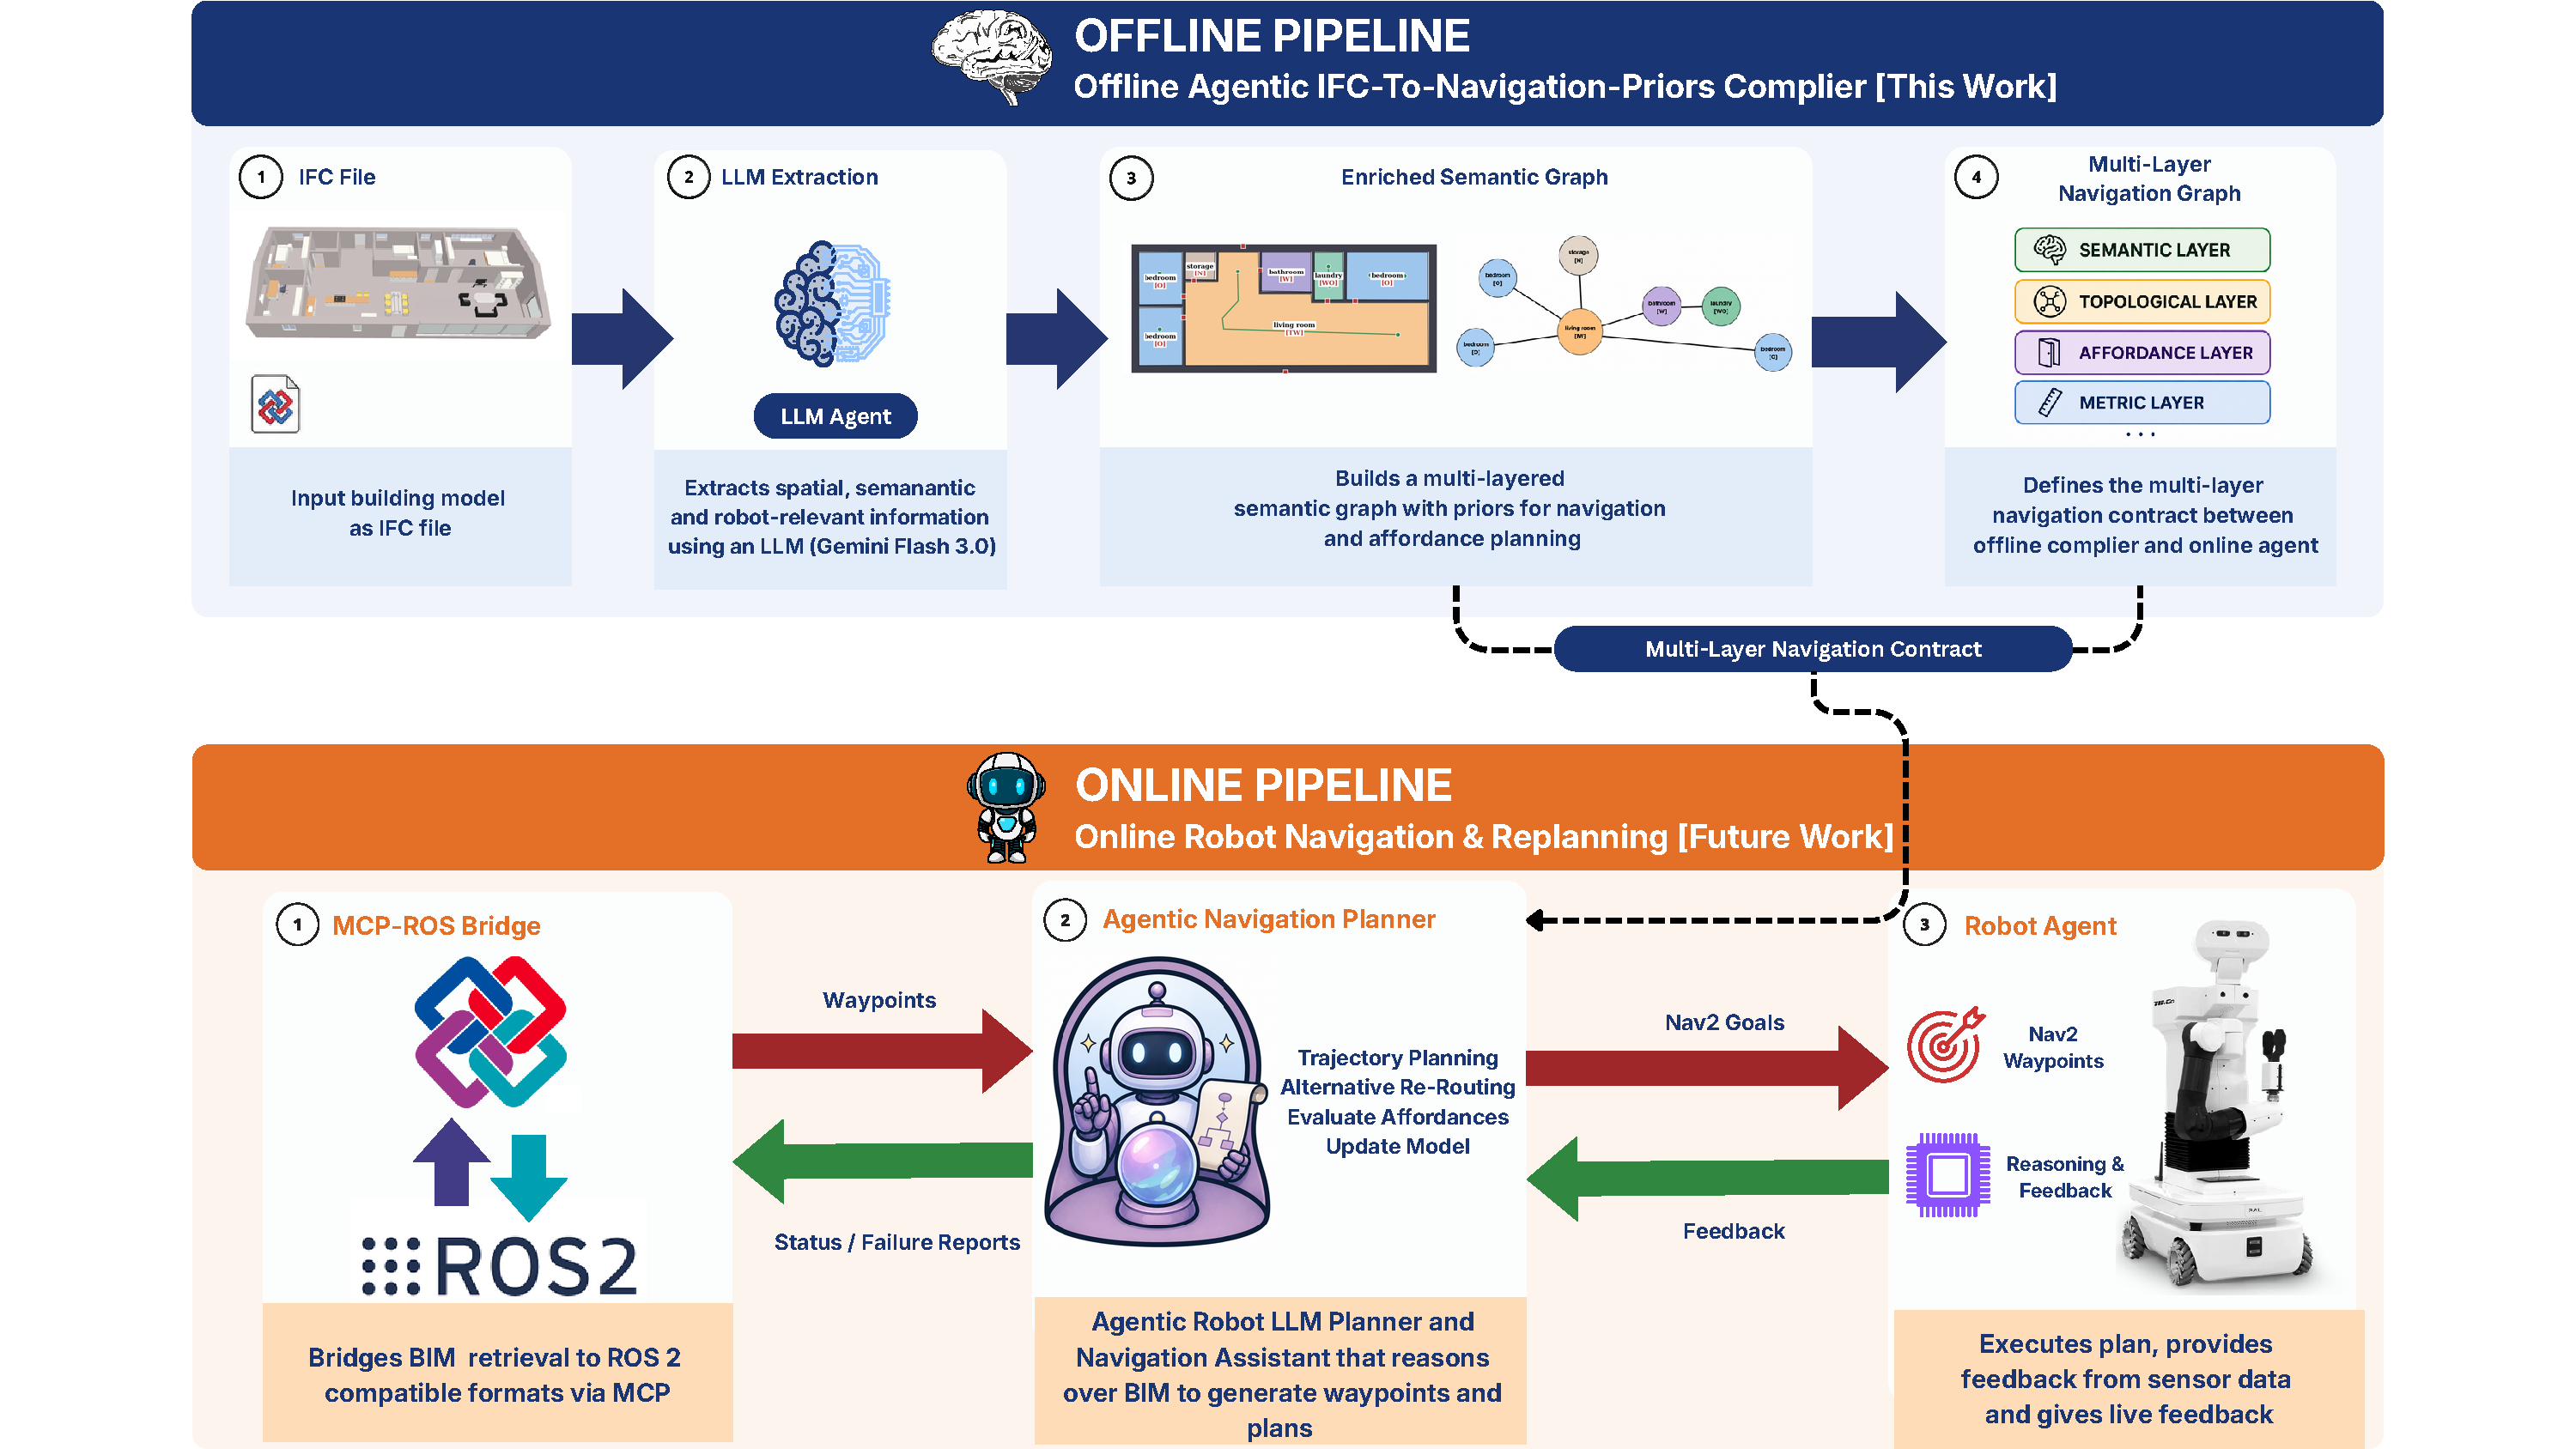
\includegraphics[width=1.0\textwidth]{figures/RoboBIM-Pipeline.pdf}
\caption{RoboBIM system overview. \textbf{Top (this paper):} The IFC model is compiled into a multi-layer navigation contract using a staged LLM agent (Gemini~3.0~Flash). This stage combines a deterministic structural backbone with a semantic enrichment layer. \textbf{Bottom (future extension, Sec.~\ref{sec:outlook}):} The navigation contract serves as input to an online agentic planner, which communicates with a ROS~2 robot agent through an MCP bridge for failure-driven replanning. This paper focuses on the offline agentic prior.}
\label{fig:system_architecture}
\end{figure*}

% ================================================================
% II. RELATED WORK
% ================================================================
\section{Related Work}

\textbf{Deterministic IFC-to-robot priors.} Existing work has shown how IFC models can be converted into robot-usable geometric and topological priors. Hamieh et al.~\cite{hamieh2021, hamieh2025} convert IFC models into weighted hypergraphs for cascaded A$^{*}$ planning. Follini et al.~\cite{follini2020} define an IFC-to-costmap pipeline, while later work~\cite{kim2021bim, kim2022semantic, constructionrobotics2023} automates waypoint extraction for construction robots. The IFC-graph literature~\cite{teo2018igit, lin2020igssnn, zhu2024graph, ifcgraph2025} further formalizes how topological graphs can be generated from IFC. These methods provide reliable structural priors, but they have a shared limitation: they can only expose semantic information that is explicitly available in the IFC schema. RoboBIM builds on this deterministic line of work. Its main contribution is an agentic enrichment layer that adds missing robot-relevant semantics on top of the deterministic backbone.

\textbf{3D scene graphs and perception-based semantic priors.} Recent systems such as SayPlan~\cite{rana2023sayplan}, EmbodiedRAG~\cite{booker2024embodiedrag}, ContextMatters~\cite{contextmatters2026}, and Taskography~\cite{agia2022taskography} build hierarchical 3D scene graphs from onboard sensing and use LLMs for high-level task planning. Ray et al.~\cite{ray2025structured} also define structured interfaces for scene-graph reasoning. These methods address a problem that is complementary to ours. They recover rich semantic information from perception when no prior map is available. RoboBIM addresses the reverse problem: it starts from an existing design-time IFC model and enriches it into a robot-ready semantic prior, without requiring perception at compile time. Pix2G~\cite{longo2025pix2g} connects these directions by combining IFC with online scene-graph construction. RoboBIM targets the upstream step: making the IFC model itself semantically rich enough to support such downstream systems.

\textbf{LLM-BIM integration for design.} Recent work shows that LLMs can interact with IFC models. MCP4IFC~\cite{nithyanantham2025mcp4ifc}, ifcMCP~\cite{lin2025ifcmcp}, modular MCP-BIM architectures~\cite{mcpbimarch2025}, and Text2BIM~\cite{du2024text2bim} use LLMs for BIM querying, editing, or generative authoring. BIM2RDT~\cite{bim2rdt2025} applies agentic reasoning to point-cloud-to-BIM alignment. Kim et al.~\cite{kim2025llmrobot} use LLMs for construction-robot task planning based on BIM data. These works demonstrate the value of LLMs for BIM reasoning, but they mainly focus on design, authoring, alignment, or downstream task planning. They do not provide a safety-constrained pipeline for compiling IFC into a robot navigation prior. RoboBIM addresses this gap by using LLMs to enrich deterministic IFC-to-robot priors while preserving the structural baseline.

\textbf{LLMs for affordance- and capability-aware planning.} Systems such as SayCan~\cite{ahn2022saycan}, AutoGPT+P~\cite{birr2024autogptp}, VAMOS~\cite{vamos2025}, TIC-VLA~\cite{huang2026ticvla}, AINav~\cite{ainav2025}, BrainBody-LLM~\cite{brainbody2025}, and IndoorR2X~\cite{indoorr2x2026} ground LLM plans in robot affordances, capabilities, and adaptive replanning. These methods focus on how a robot should act once a semantic prior is available. RoboBIM addresses the earlier step: it creates the navigation contract that can serve as input to such planners.

\textbf{Positioning.} Table~\ref{tab:gap} summarizes this research landscape. RoboBIM differs from prior work in three main ways. First, it uses staged LLM inference instead of a single monolithic LLM call. Second, it includes an explicit topology regression gate to protect the deterministic structural baseline. Third, it produces a multi-consumer navigation contract rather than a single task-specific output format.

\begin{table}[t]
\centering
\caption{\textbf{Positioning.} RoboBIM focuses on agentic IFC-to-prior compilation. This direction is complementary to deterministic IFC pipelines and perception-based semantic-prior methods.}
\label{tab:gap}
\footnotesize
\setlength{\tabcolsep}{3pt}
\begin{tabularx}{\columnwidth}{@{}X c c c@{}}
\toprule
\textbf{Capability} & \makecell{\textbf{Det.}\\\textbf{IFC}} & \makecell{\textbf{3DSG +}\\\textbf{LLM}} & \textbf{RoboBIM} \\
\midrule
IFC as prior source             & \cmark & \xmark & \cmark \\
Rich semantic annotation        & \xmark & \cmark & \cmark \\
No perception required          & \cmark & \xmark & \cmark \\
Staged LLM with bounded roles   & \xmark & partial & \cmark \\
Topology regression gate        & \xmark & \xmark & \cmark \\
Multi-consumer contract         & partial & \xmark & \cmark \\
Per-robot traversability        & \xmark & partial & \cmark \\
\bottomrule
\end{tabularx}
\end{table}

% ================================================================
% III. METHODOLOGY
% ================================================================
\section{Methodology}
\label{sec:method}

The RoboBIM system has two main parts: a deterministic geometric backbone and an LLM agent wrapper, as shown in Fig.~\ref{fig:pipeline}. The backbone takes one IFC file as input and produces the static graph $\mathcal{G}_{\text{static}}=(\mathcal{O},\mathcal{W},\mathcal{T})$. This graph contains per-storey occupancy grids $\mathcal{O}$, a clearance-aware waypoint graph $\mathcal{W}$, and a room-transition topology $\mathcal{T}$. The LLM agent wrapper runs seven stages on top of the same backbone. It inspects the IFC file through a sandboxed Python interpreter, and adds semantic fields $\Sigma$ to the graph. These fields include room types, hazards, materials, traversability, and building-level policies. The final output is the enriched graph $\mathcal{G}_{\text{agent}}=(\mathcal{O},\mathcal{W},\mathcal{T},\Sigma)$. RoboBIM exports this graph to Nav2, Open-RMF, GraphML, and GeoJSON. It also produces a deterministic natural-language briefing that can ground onboard robot LLMs. Appendix~\ref{app:stages} provides the stage specifications, prompts, clamp ranges, and confidence-threshold tables.

\subsection{Deterministic backbone}

The backbone is a five-module pipeline. First, the loader extracts storeys, doors, and \texttt{IfcSpace} entities from the IFC file. Second, the occupancy module rasterizes walls and columns into a 5\,cm grid for each storey. Third, the segmentation module computes a Euclidean signed distance field, extracts a generalized Voronoi diagram (GVD) skeleton, and labels rooms using door-aware connected components. If no \texttt{IfcSpace} entities are available, it falls back to a purely geometric segmentation. Fourth, the waypoint module traces the skeleton into a sparse graph. It also injects door-crossing waypoints so that the graph follows the building's access topology. Finally, the topology module builds the room-transition graph, attaches material information from property sets, and checks cross-storey consistency. This check flags stair or elevator transitions whose endpoints do not align across floors. The resulting $\mathcal{G}_{\text{static}}$ is produced without LLM intervention and serves as the safety baseline.


\subsection{Agentic enrichment layer}

The agent wrapper adds seven stages. Each stage reads from and writes to a shared Pipeline Context. Stage~0 explores the IFC file through a sandboxed Python tool backed by \texttt{IfcOpenShell}~\cite{ifcopenshell}. The tool uses a hard timeout, blocks file writes, and disallows unsafe imports. Stage~1 produces extraction hyperparameters, including grid resolution, dilation radius, minimum room area, door search radius, and the include-openings flag for the deterministic backbone. These parameters are controlled by a policy in $\{\texttt{apply}, \texttt{suggest}, \texttt{fixed}\}$, with \texttt{fixed} as the default. Stage~2 infers room types. A regex and property-set prefilter first resolves deterministic cases. The remaining rooms on each storey are then sent to the LLM in a single batched prompt, which gives the model cross-room context. For example, an unlabelled space with multiple door transitions and adjacent office-labelled rooms can be inferred as a corridor. This type of regularity is difficult to encode with fixed rules but is easier to infer in context. Stage~2b reviews the segmentation and may issue merge directives. Merge directives with confidence $\geq 0.70$ are applied, while split suggestions are recorded but not applied. Stage~3 validates connectivity and proposes add, remove, or reclassify edits. A topology regression gate then audits the connected-transition count and rolls back any edit that reduces it below the deterministic baseline. Stage~4 writes hazards (controlled vocabulary $\{$wet area, narrow passage, fall risk, high traffic, obstacle dense, restricted access$\}$), floor materials, and a traversability score in the range $[0,1]$. Stage~5 produces a natural-language audit and briefing. This briefing is designed to be copied directly into the system prompt of an onboard robot LLM, so the robot does not need runtime access to the IFC file.

\begin{figure}[hbt!]
\centering
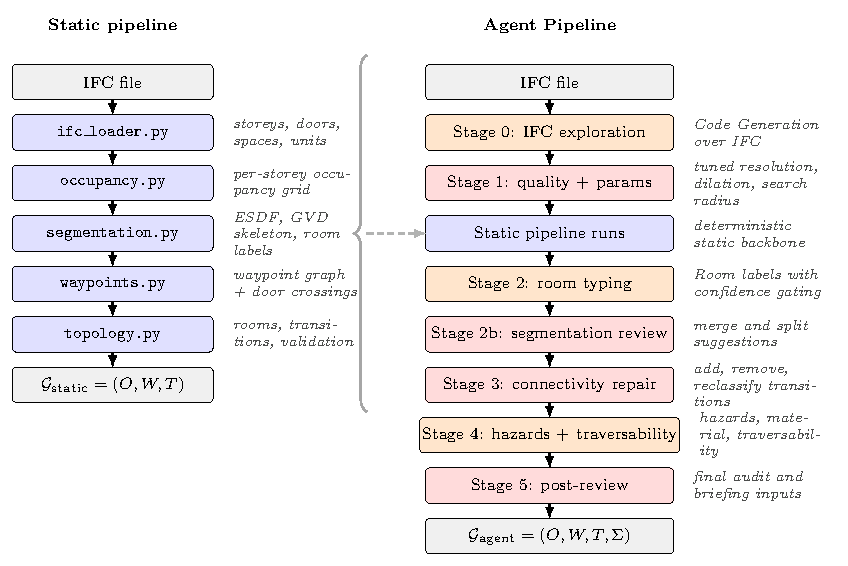
\includegraphics[width=\columnwidth]{figures/pipeline.pdf}
\vspace{-4pt}
\caption{Static pipeline (left) vs RoboBIM agent pipeline (right). The static pipeline is five deterministic Python modules that produce $\mathcal{G}_{\mathrm{static}}$. The agent pipeline wraps the same backbone with seven LLM stages and a topology regression gate, producing $\mathcal{G}_{\mathrm{agent}}=(\mathcal{O},\mathcal{W},\mathcal{T},\Sigma)$.}
\label{fig:pipeline}
\end{figure}


\subsection{Output graph}

The enriched graph $\mathcal{G}_{\text{agent}}$ has three linked layers. Appendix Fig.~\ref{fig:layers} shows these layers on \texttt{BasicHouse}. Layer~1 is a per-storey occupancy grid with 5\,cm resolution. Each cell is labelled as free, occupied, or unknown. Layer~2 is a per-storey waypoint graph derived from the GVD skeleton. Each edge stores a clearance value $c\in\mathbb{R}_{\geq 0}$, which determines whether a robot with inflated radius $r$ can traverse the edge, i.e., $c\geq r$. Layer~3 is a topological graph of rooms and transitions, including doors, wall openings, and stair or elevator landings. The layers are connected through explicit cross-layer links. Each room is linked to its waypoint cluster, and each transition is linked to its crossing waypoint. These links support hierarchical planning, from a room-level topological plan to a metric trajectory. The deterministic baseline reserves per-room semantic fields but leaves them empty. These fields include the room type label with confidence and source, hazard list, floor-material string, and traversability score in $[0,1]$. The agentic layer populates these fields. It also derives building-level policies, such as the tightest door-width invariant and non-navigable storeys. These policies are attached to the graph rather than to a single room.

% ================================================================
% IV. EXPERIMENTS
% ================================================================
\section{Experiments}

\begin{table*}[!t]
\centering
\caption{Per-building results on four IFC models. The Geometry columns are identical for both pipelines (the gate forbids regression) and listed once. Semantic enrichment columns are written \mbox{static~$\rightarrow$~agent}.}
\label{tab:coverage}
\footnotesize
\setlength{\tabcolsep}{4.0pt}
\begin{tabular}{@{}l c c c c | c c c c c | r r@{}}
\toprule
& \multicolumn{4}{c|}{Geometry (preserved)}
  & \multicolumn{5}{c|}{Semantic enrichment (static~$\rightarrow$~agent)}
  & \multicolumn{2}{c}{Agent cost} \\
Model & storeys & rooms & conn.\ trans. & waypoints
    & type & w/ hazard & traversability & material & policy
    & time (s) & tok.\ in/out \\
\midrule
4351          & 5  & 22  & 10 & 90  & $1\!\rightarrow\!1$    & $0\!\rightarrow\!3$  & $0\!\rightarrow\!22$  & $0\!\rightarrow\!5$  & $0\!\rightarrow\!5$ & 294  & 285k/32k \\
BasicHouse    & 2  & 14  & 6  & 32  & $0\!\rightarrow\!7$    & $0\!\rightarrow\!7$  & $0\!\rightarrow\!14$  & $0\!\rightarrow\!7$  & $0\!\rightarrow\!6$ & 489  & 200k/24k \\
digital\_hub  & 3  & 64  & 60 & 304 & $38\!\rightarrow\!64$  & $0\!\rightarrow\!0$  & $0\!\rightarrow\!64$  & $0\!\rightarrow\!0$  & $0\!\rightarrow\!1$ & 423  & 343k/32k \\
macalister    & 6  & 31  & 9  & 392 & $12\!\rightarrow\!17$  & $0\!\rightarrow\!9$  & $0\!\rightarrow\!31$  & $0\!\rightarrow\!17$ & $0\!\rightarrow\!6$ & 407  & 348k/41k \\
\midrule
\textbf{total} & \textbf{16} & \textbf{131} & \textbf{85} & \textbf{818} & $\mathbf{51\!\rightarrow\!89}$ & $\mathbf{0\!\rightarrow\!19}$ & $\mathbf{0\!\rightarrow\!131}$ & $\mathbf{0\!\rightarrow\!29}$ & $\mathbf{0\!\rightarrow\!18}$ & 1612 & 1176k/129k \\
\bottomrule
\end{tabular}
\end{table*}

\subsection{Setup}
For the preliminary results, we evaluate RoboBIM on four public IFC models from IFC Bench~\cite{ifc_repo}: \texttt{4351}, \texttt{BasicHouse}, \texttt{digital\_hub}, and \texttt{samuel\_macalister\_sample\_house}. These models cover residential, mixed-use, and office layouts, with 14-64 rooms across 2-6 storeys. \texttt{BasicHouse} contains no \texttt{IfcSpace} entities and is therefore used to test the geometric fallback. Appendix~\ref{app:corpus} reports the licenses, and raw element counts for all models. We run both the deterministic backbone and the full agent pipeline using Gemini~3.0~Flash on each building. Each reported value is based on a single run, and we discuss this limitation in Sec.~\ref{sec:outlook}. We compare the two settings along three axes: the geometric graph, the populated semantic fields, and the wall-clock and token cost of the agent pass.

\subsection{Results}
Table~\ref{tab:coverage} summarizes the results for each IFC model. Across the full corpus, room-type coverage increases from 51 to 89 out of 131 rooms (an increase of +74.5\%). The deterministic baseline leaves hazard, traversability, material, and policy fields empty, while the agentic output populates these fields. On \texttt{BasicHouse}, which has no \texttt{IfcSpace} entities, the agent labels all 7 navigable rooms using only geometry and adjacency. It also infers hazards for kitchen, bathroom, and laundry areas. On \texttt{digital\_hub}, the agent closes the 38-of-64 gap left by the regex prefilter and reaches full room-type coverage. No agent-proposed edit reduced the connected-transition count below the deterministic baseline in any of the four runs.

Agent wall-clock time ranges from 294 to 489\,s per IFC model, with a mean of 403\,s. Input token usage ranges from 200\,k to 348\,k, and output token usage ranges from 24\,k to 41\,k. Per-storey batching keeps the number of LLM calls between 7 and 15 per run. Stage~0 and Stage~2 account for most of the runtime. Stage~2b is the main cost on \texttt{BasicHouse}, where the geometric fallback is used. Stage~3 is the main cost on \texttt{digital\_hub}, which has the densest connectivity graph. Appendix~\ref{app:perifc} reports the per-stage breakdowns in Fig.~\ref{fig:cost} and Tables~\ref{tab:per_ifc_usage}.

\subsection{Qualitative analysis and online query agent (motivation)}
A qualitative comparison on Floor~0 of \texttt{BasicHouse} is shown in Appendix Fig.~\ref{fig:hero}. The static pipeline outputs grey rooms with only geometric indices. In contrast, the agent output colours rooms by inferred type, including \texttt{living\_room}, \texttt{bedroom}, \texttt{bathroom}, \texttt{laundry}, and \texttt{storage}. It also shows hazard codes: $W$ for wet area, $O$ for obstacle-dense area, $T$ for high-traffic area, and $N$ for narrow passage. Listing~\ref{lst:brief} in the appendix shows a four-room excerpt from the generated briefing. The excerpt includes room type, hazards, material, traversability, and derived navigation policies, such as the tightest door width of 0.91\,m, a robot width limit of 0.81\,m, caution rooms, and non-navigable storeys. These fields are not populated by the deterministic baseline. The exports and briefing can be provided to a robot-side LLM through the Model Context Protocol~\cite{anthropic2024mcp}. For example, when the local planner reports a blocked door or occluded corridor, an onboard agent can query alternatives that satisfy width, hazard, and traversability constraints. This allows the robot to replan using the prior instead of re-exploring the full global state space. We leave the empirical evaluation of this online loop to future work.

% ================================================================
% V. CONCLUSION & FUTURE WORK
% ================================================================
\section{Conclusion and Future Work}
\label{sec:outlook}

We presented RoboBIM, an IFC-to-navigation-graph pipeline that enriches a deterministic geometric backbone with robot-relevant semantics. On four public buildings, the agent increases room-type coverage by 74.5\%, fills hazard, material, traversability, and policy fields that are empty in the baseline, and preserves connected topology in every run. The current study has three main limitations: the results are based on single-run measurements, the topology gate checks only connected-transition count, and the confidence thresholds are chosen heuristically. Future work will address these limitations in three directions. First, we will study the gap between as-designed and as-built environments by fusing perception with the prior. In this setting, $\mathcal{G}_{\text{agent}}$ can serve as a stable reference target for Hydra-class systems~\cite{hughes2024hydra}, with updates supported by DAAAM-style captions~\cite{gorlo2025daaam}. Second, we will stress-test the regression gate with synthetic bad-merge prompts. Third, we will evaluate the online query agent from Fig.~\ref{fig:system_architecture} in end-to-end ROS~2 deployments.

% ================================================================
% REFERENCES
% ================================================================
\bibliographystyle{ieeetr}
{\footnotesize
\bibliography{references}}

% ================================================================
% APPENDIX
% ================================================================
\appendix

\section{Agent Stage Specification}
\label{app:stages}

This appendix expands the seven agent stages introduced in Section~\ref{sec:method}. For each stage we describe the inputs it reads, the output it produces, and the conditions under which its proposals are written back into the graph.

\subsection{Stage 0: building exploration}
The agent receives a compact summary of the input building file that lists entity counts, storeys, doors, and representative property sets. It is also given a sandboxed Python runner with read-only access to the loaded building model through IfcOpenShell~\cite{ifcopenshell}. The runner enforces a hard timeout and blocks imports of non-standard libraries and file writes. The agent responds with free-form findings, which are parsed into evidence items and stored in the Pipeline Context.

\subsection{Stage 1: quality analysis and parameter tuning}
The agent reads the building summary together with the Stage 0 findings. It returns a structured object with a completeness score, a recommended strategy, and five numeric parameters: grid resolution, dilation radius, minimum room area, door search radius, and an include-openings flag. All numeric parameters are clamped to safe ranges. A parameter policy controls the write-back behaviour. In the apply mode, the parameters are used directly. In the suggest mode, they are used only if they lie inside the clamp range. In the fixed mode, which is the default, they are logged but not used.

\subsection{Stage 2: room-type inference}
A regex prefilter types rooms with obvious names, such as corridor, CX, or WC. An element-set prefilter handles rooms with matching content, a room with two or more sanitary terminals is treated as a bathroom. Rooms resolved by either prefilter skip the LLM. The remaining rooms on a given storey are sent to the LLM in a single batched prompt. A newly assigned type requires a confidence of at least $0.80$, and overriding an existing type requires a confidence of at least $0.75$.

\subsection{Stage 2b: segmentation review}
The agent reads the room list and the transitions, then proposes merge or split directives. Merges with a confidence of at least $0.70$ are applied at the topology layer: the bounding boxes are combined, the transitions are reassigned, and the absorbed room is removed. Split directives are recorded only, because they require label-map access that is not preserved after extraction.

\subsection{Stage 3: connectivity validation and repair}
The agent produces a list of issues, such as isolated rooms or suspicious connections. It then outputs a repair plan with three directive kinds: \texttt{add\_connection}, \texttt{remove\_connection}, and \texttt{reclassify}. Directives with a confidence of at least $0.70$ are applied. The topology regression gate then checks the resulting connected-transition count, and any edit that reduces it is rolled back.

\subsection{Stage 4: hazards and traversability}
For each room, the agent writes a list of hazard flags from a controlled vocabulary, a floor-material string, a traversability score in $[0, 1]$, a short robot-obstacles string, and a prose note. The stage reuses the prefilter and the per-storey batching introduced in Stage 2.

\subsection{Stage 5: post-extraction review}
The agent reads the final enriched graph and returns a short audit that contains an overall quality score, a completeness score, a gaps list, and improvement suggestions. The audit is stored in the Pipeline Context and is used as input to the natural-language briefing.

\section{Output Graph Visualisation}
\label{app:layers}

\begin{figure}[h]
\centering
\begin{subfigure}[b]{0.48\columnwidth}
  \centering
  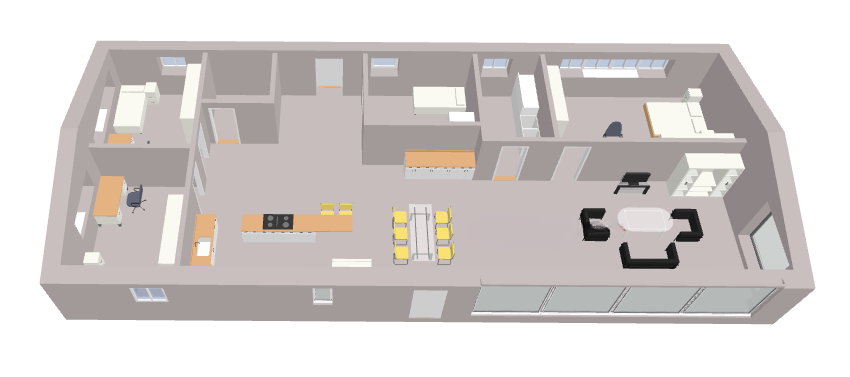
\includegraphics[width=\linewidth,height=2.5cm,keepaspectratio]{figures/BasicHouse_fixed.png}
  \caption{Input IFC file.}
\end{subfigure}\hfill
\begin{subfigure}[b]{0.48\columnwidth}
  \centering
  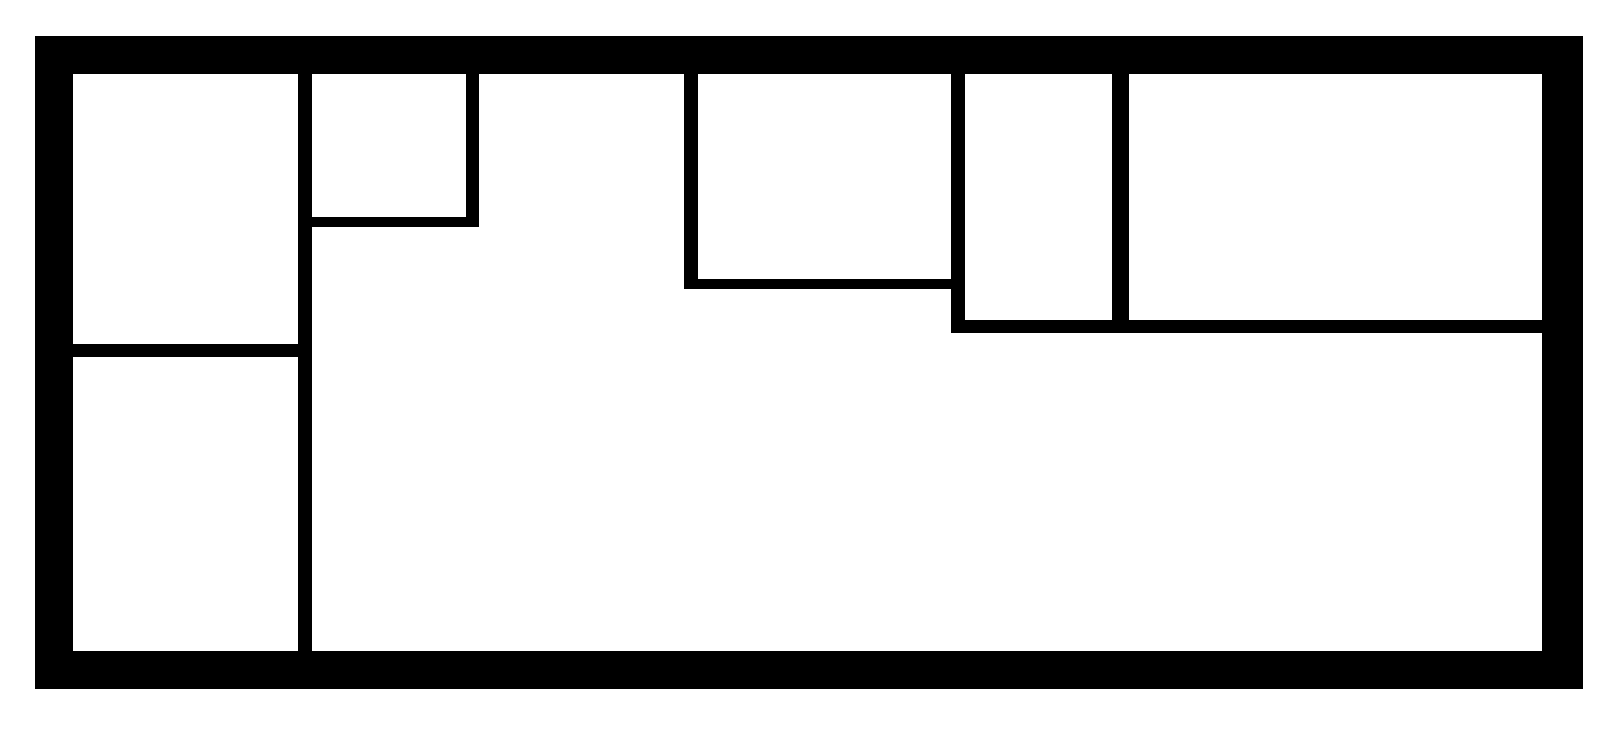
\includegraphics[width=\linewidth,height=2.5cm,keepaspectratio]{figures/fig_layer1_occupancy.png}
  \caption{Layer 1: occupancy.}
\end{subfigure}

\vspace{2pt}
\begin{subfigure}[b]{0.48\columnwidth}
  \centering
  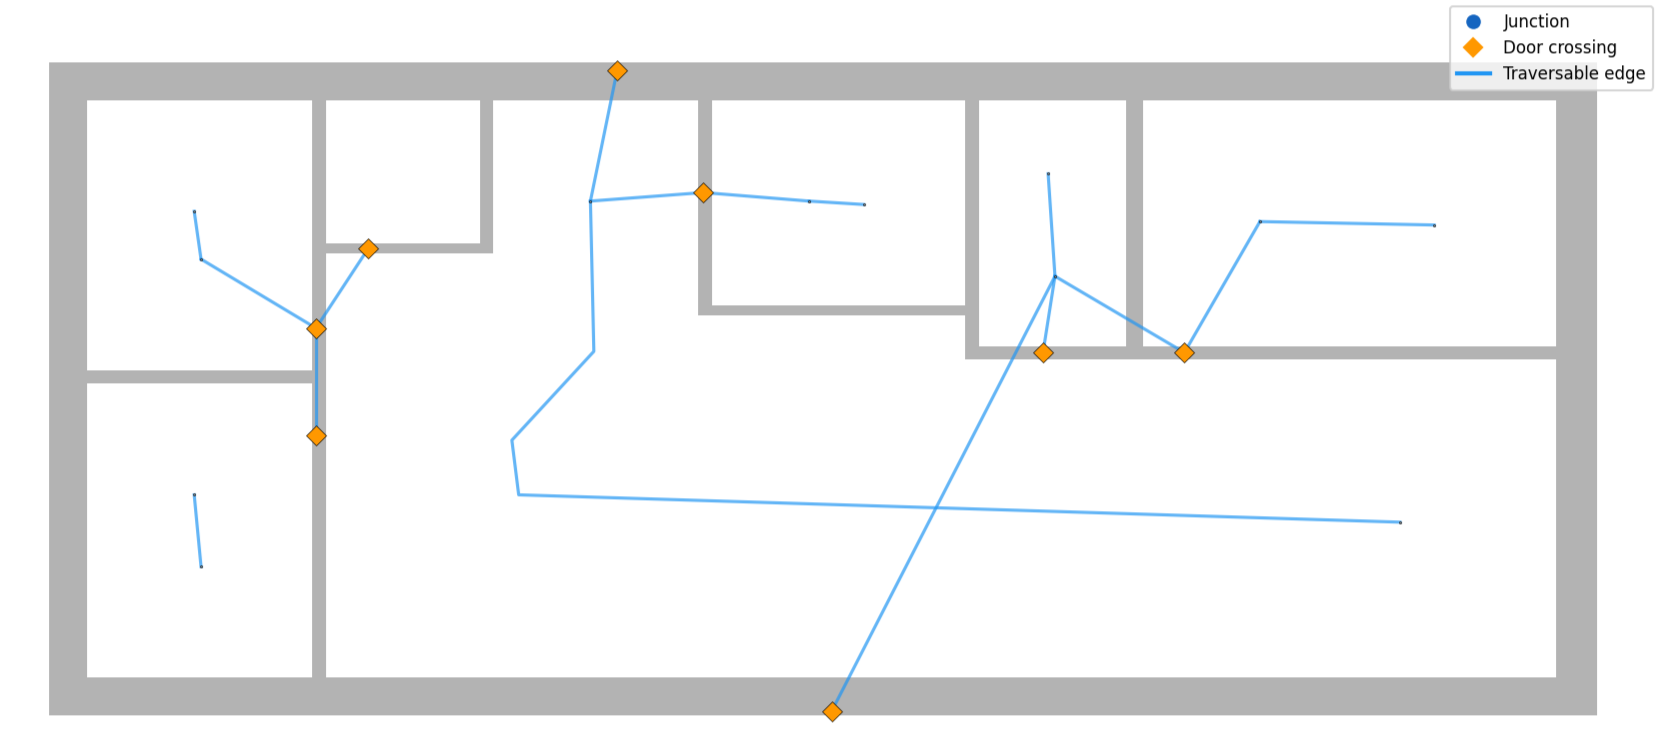
\includegraphics[width=\linewidth,height=2.5cm,keepaspectratio]{figures/fig_layer2_waypoints.png}
  \caption{Layer 2: waypoints.}
\end{subfigure}\hfill
\begin{subfigure}[b]{0.48\columnwidth}
  \centering
  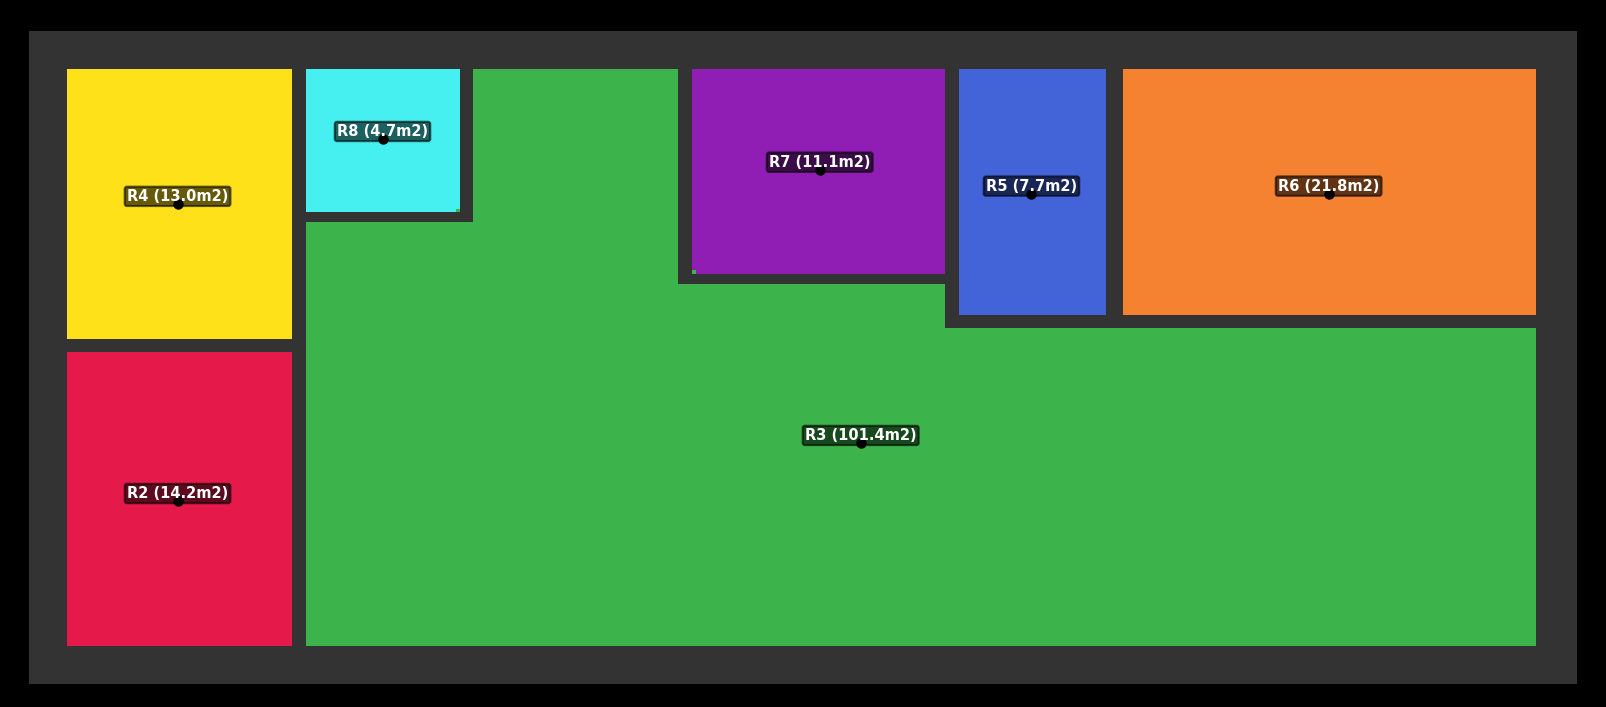
\includegraphics[width=\linewidth,height=2.5cm,keepaspectratio]{figures/fig_layer3_rooms.png}
  \caption{Layer 3: rooms.}
\end{subfigure}
\vspace{-4pt}
\caption{Input IFC file and the three linked layers on \texttt{BasicHouse}, ground floor. Top-left: input IFC rendering. Top-right: Layer 1, 5\,cm occupancy grid. Bottom-left: Layer 2, GVD-derived waypoint graph with clearance-annotated edges. Bottom-right: Layer 3, room-and-transition topology. Cross-layer links (not drawn) connect each room to its waypoint cluster and each door to its crossing waypoint.}
\label{fig:layers}
\end{figure}

\begin{figure}[h]
\centering
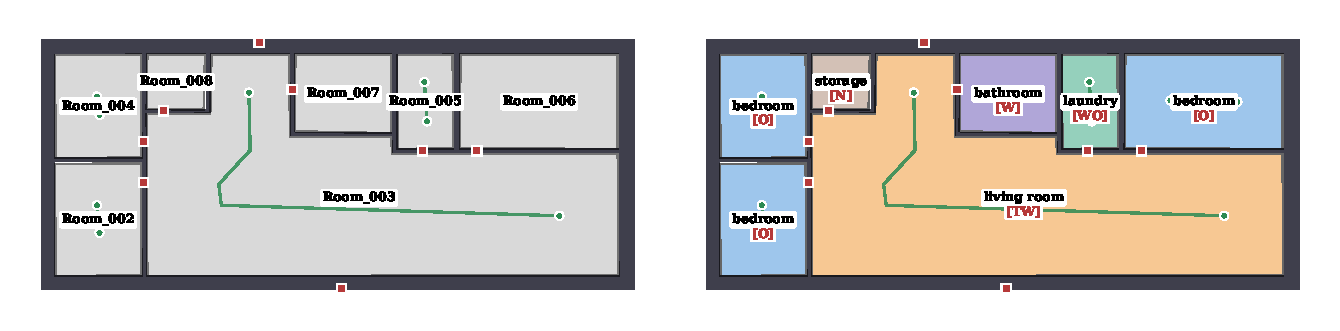
\includegraphics[width=\columnwidth]{figures/fig_hero_floorplan.pdf}
\vspace{-4pt}
\caption{Floor 0 in \texttt{BasicHouse}. Left: static output. Right: agent output. Rooms coloured by inferred type with hazard codes in brackets ($W$=wet, $O$=obstacle-dense, $T$=high traffic, $N$=narrow).}
\label{fig:hero}
\end{figure}

\section{Corpus Sources and Properties}
\label{app:corpus}

The four building models used in the main evaluation are all public and redistributable, and each is taken directly from its original repository. \texttt{4351}\footnote{\url{https://github.com/opensourceBIM/TestFiles}} and \texttt{samuel\_macalister\_sample\_house}\footnote{\url{https://github.com/opensourceBIM/TestFiles}} come from the BIMserver TestFiles collection. \texttt{digital\_hub}\footnote{\url{https://github.com/RWTH-E3D/DigitalHub}} comes from the RWTH E3D DigitalHub release. \texttt{BasicHouse}\footnote{\url{https://github.com/andrewisen/bim-whale-ifc-samples/tree/master/BasicHouse}} comes from the BIM-Whale samples repository. Together, these sources span several design disciplines and both major revisions of the IFC file format.

Table~\ref{tab:corpus_sources} lists the upstream origin, the license, and the intended building use for each model. Table~\ref{tab:corpus_stats} lists raw statistics extracted from each file: the schema version, the on-disk file size, and the total counts of storeys, doors, rooms, and walls. These counts are independent of our pipeline and reflect the authoring state of each file.

\begin{table}[h]
\centering
\caption{Provenance of each building model in the corpus.}
\label{tab:corpus_sources}
\footnotesize
\setlength{\tabcolsep}{3pt}
\begin{tabular}{@{}l l l l@{}}
\toprule
Model & Upstream source & License & Use \\
\midrule
4351         & BIMserver TestFiles   & GPL v3 & office \\
BasicHouse   & BIM-Whale Samples     & MIT    & residential \\
digital\_hub & RWTH E3D DigitalHub   & MIT    & mixed-use \\
macalister   & BIMserver TestFiles   & GPL v3 & residential \\
\bottomrule
\end{tabular}
\end{table}

\begin{table}[h]
\centering
\caption{Raw building-file statistics extracted from each model. The rooms column shows how many rooms are explicitly annotated by the author; a zero means the pipeline must recover rooms geometrically.}
\label{tab:corpus_stats}
\footnotesize
\setlength{\tabcolsep}{3pt}
\begin{tabular}{@{}l l r r r r r@{}}
\toprule
Model & Schema & Size (MB) & Storeys & Doors & Rooms & Walls \\
\midrule
4351         & IFC2X3 & 7.3  & 5 & 17 & 6  & 43  \\
BasicHouse   & IFC2X3 & 51.7 & 2 & 8  & 0  & 13  \\
digital\_hub & IFC4   & 9.0  & 3 & 64 & 64 & 178 \\
macalister   & IFC4   & 25.4 & 6 & 16 & 14 & 48  \\
\bottomrule
\end{tabular}
\end{table}

\texttt{digital\_hub} is the densest building in the corpus, with 64 annotated rooms and 64 doors on three storeys, and tests the pipeline on a richly annotated model. \texttt{4351} is a 5-storey office with only 6 rooms annotated, so the agent must infer room types on a partially annotated file. \texttt{BasicHouse} has no room annotations at all, so segmentation falls through to the geometric GVD pass described in Section~\ref{sec:method}; it is also the largest file on disk, because it carries detailed geometry for a small floor plan. \texttt{samuel\_macalister\_sample\_house} is a 6-storey residential model with mechanical and plumbing content, and stresses the cross-storey consistency check.

\section{Per-IFC Detailed Cost Breakdown}
\label{app:perifc}

Fig.~\ref{fig:cost} stacks the seven stage timings per building and overlays the input-token count on a secondary axis. Stage 0 is always the first LLM stage; its time scales with the complexity of the input file, because the agent controls how many code-execution snippets to issue. Stage 2 (room-type inference) scales with the storey count, because it is batched per storey. Stage 2b (segmentation review) is the largest single cost on \texttt{BasicHouse}, where the lack of annotated rooms forces a richer geometric review. Stage 3 is the largest cost on \texttt{digital\_hub}, which has the densest connectivity graph in the corpus.

\begin{figure}[h]
\centering
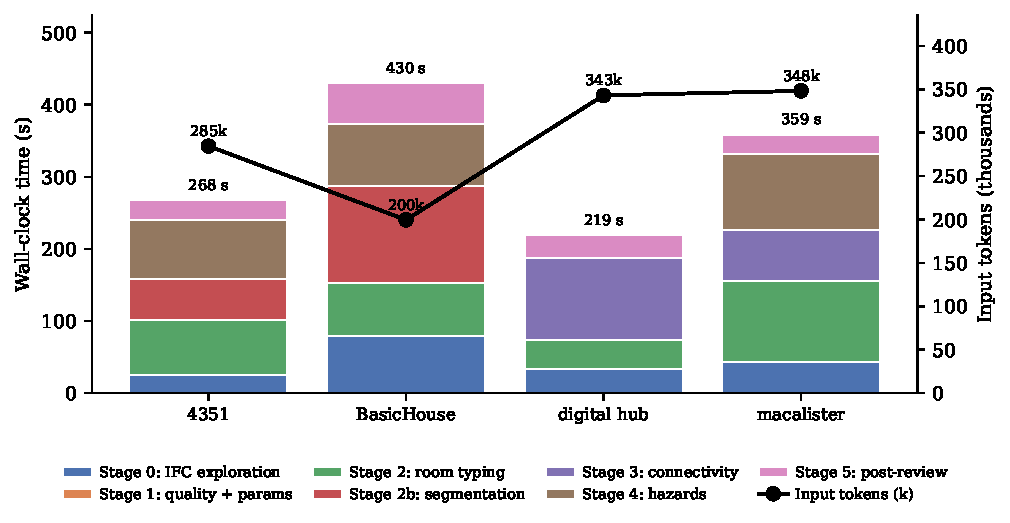
\includegraphics[width=\columnwidth]{figures/fig_stage_cost.pdf}
\vspace{-4pt}
\caption{Per-IFC agent wall-clock time stacked by stage (bars, left axis), with the input-token count overlaid as a black line (right axis). Stage 0, Stage 2, Stage 2b, and Stage 4 dominate the time budget. Confidence-gated per-storey batching keeps the total LLM call count between 7 and 15 per run.}
\label{fig:cost}
\end{figure}

Table~\ref{tab:per_ifc_usage} reports the LLM usage per building. Both the call count and the token usage are dominated by Stage 2 and Stage 4 on the smaller buildings. On \texttt{BasicHouse}, Stage 0 dominates, because the agent chose to issue more exploration snippets than on the other three buildings.

\begin{table}[h]
\centering
\caption{LLM usage per building.}
\label{tab:per_ifc_usage}
\footnotesize
\setlength{\tabcolsep}{3.4pt}
\begin{tabular}{@{}l r r r r@{}}
\toprule
Model & LLM calls & Code execs & Tokens in (k) & Tokens out (k) \\
\midrule
4351        & 13 & 28 & 285 & 32 \\
BasicHouse  &  9 & 15 & 200 & 24 \\
digital\_hub&  7 & 16 & 343 & 32 \\
macalister  & 15 & 27 & 348 & 41 \\
\midrule
total       & 44 & 86 & 1176 & 129 \\
\bottomrule
\end{tabular}
\end{table}

\section{Additional Per-Storey Qualitative Outputs}
\label{app:qualitative}

This appendix collects additional per-storey visualisations produced by the agent pipeline on two of the four buildings. Each panel is a composite view written by the pipeline that overlays the occupancy grid, the waypoint graph, and the room segmentation on a single storey.

Fig.~\ref{fig:dh_storeys} shows the three storeys of \texttt{digital\_hub}. The building has annotated rooms on every floor, so the segmentation follows the authored partitions and the waypoint graph densifies cleanly around the shared corridor on each level.

\begin{figure}[htb]
\centering
\begin{subfigure}[b]{\columnwidth}
  \centering
  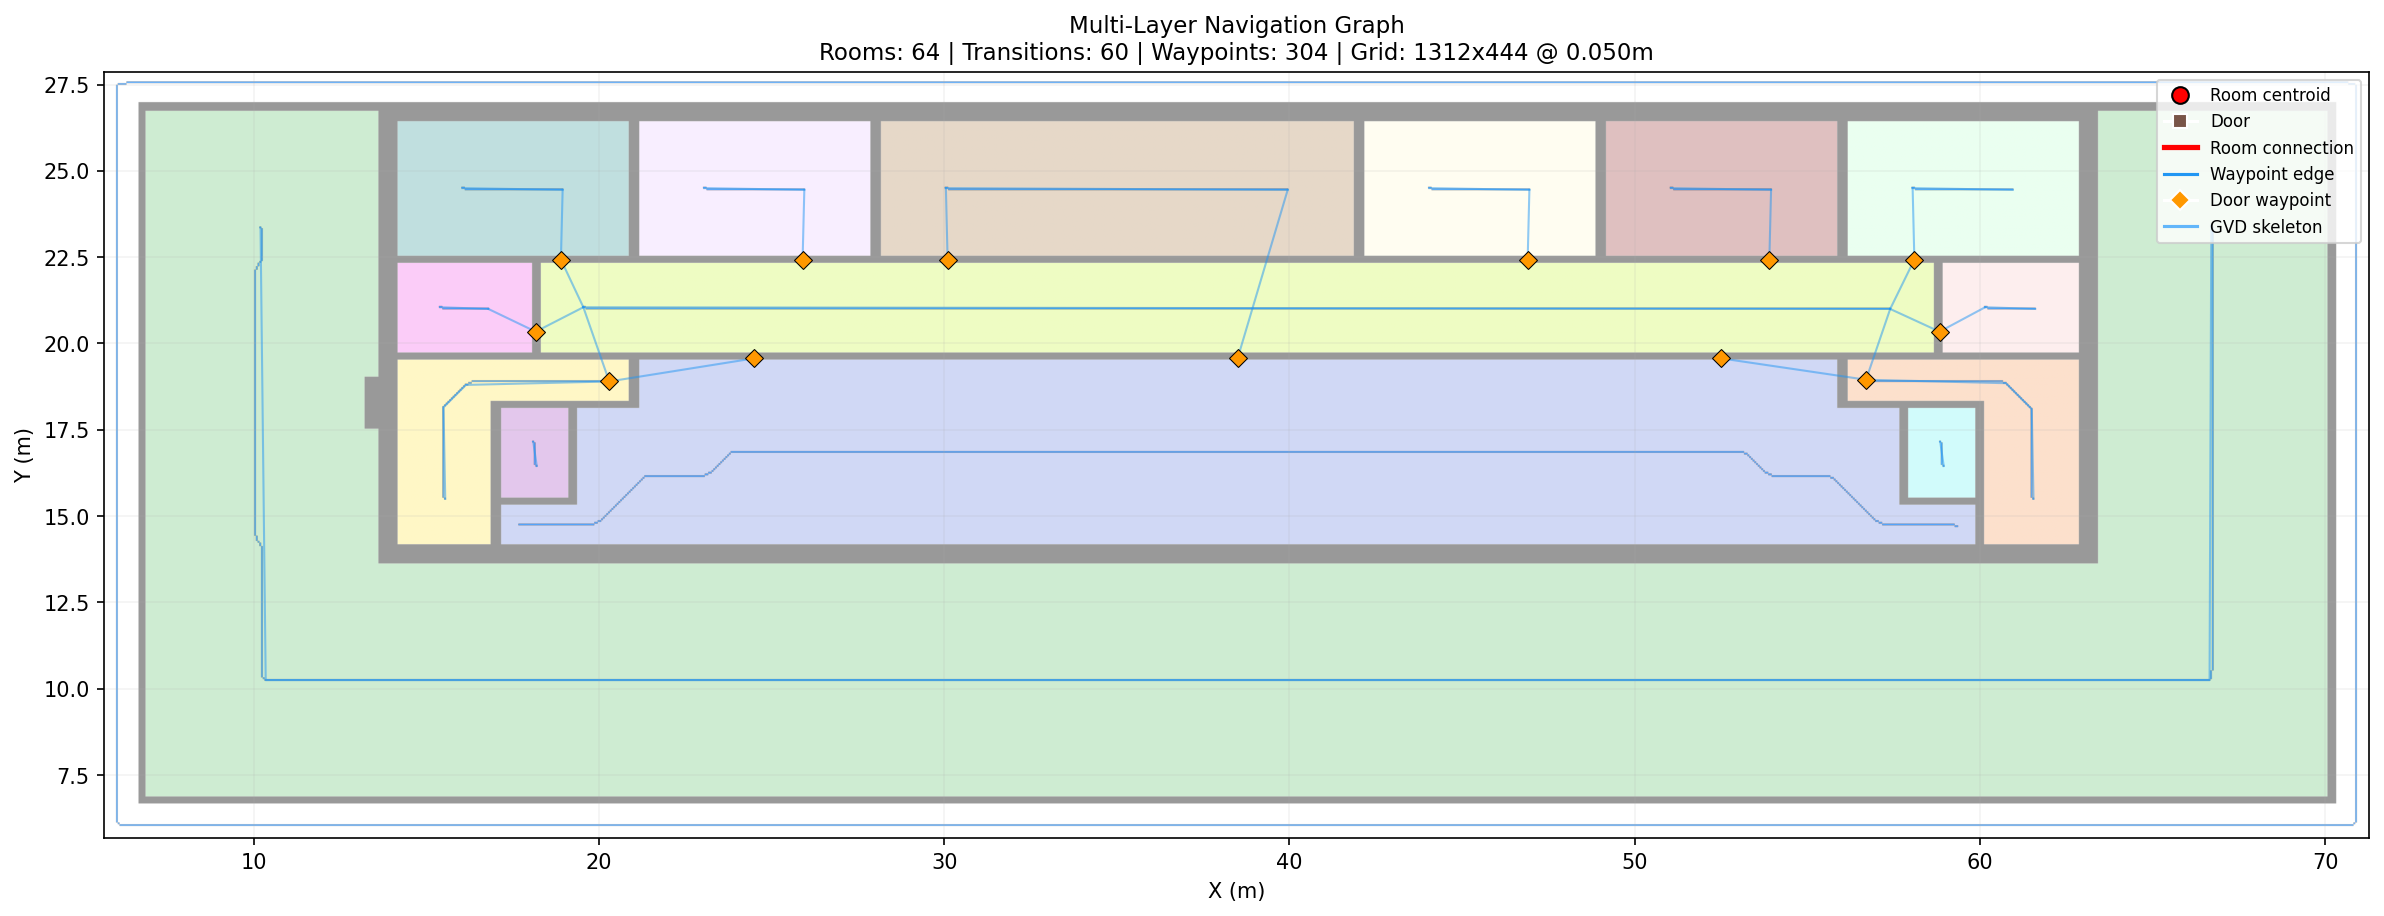
\includegraphics[width=0.95\linewidth]{figures/fig_dh_basement.png}
  \caption{Basement (B01\_OKRD).}
\end{subfigure}\vspace{2pt}
\begin{subfigure}[b]{\columnwidth}
  \centering
  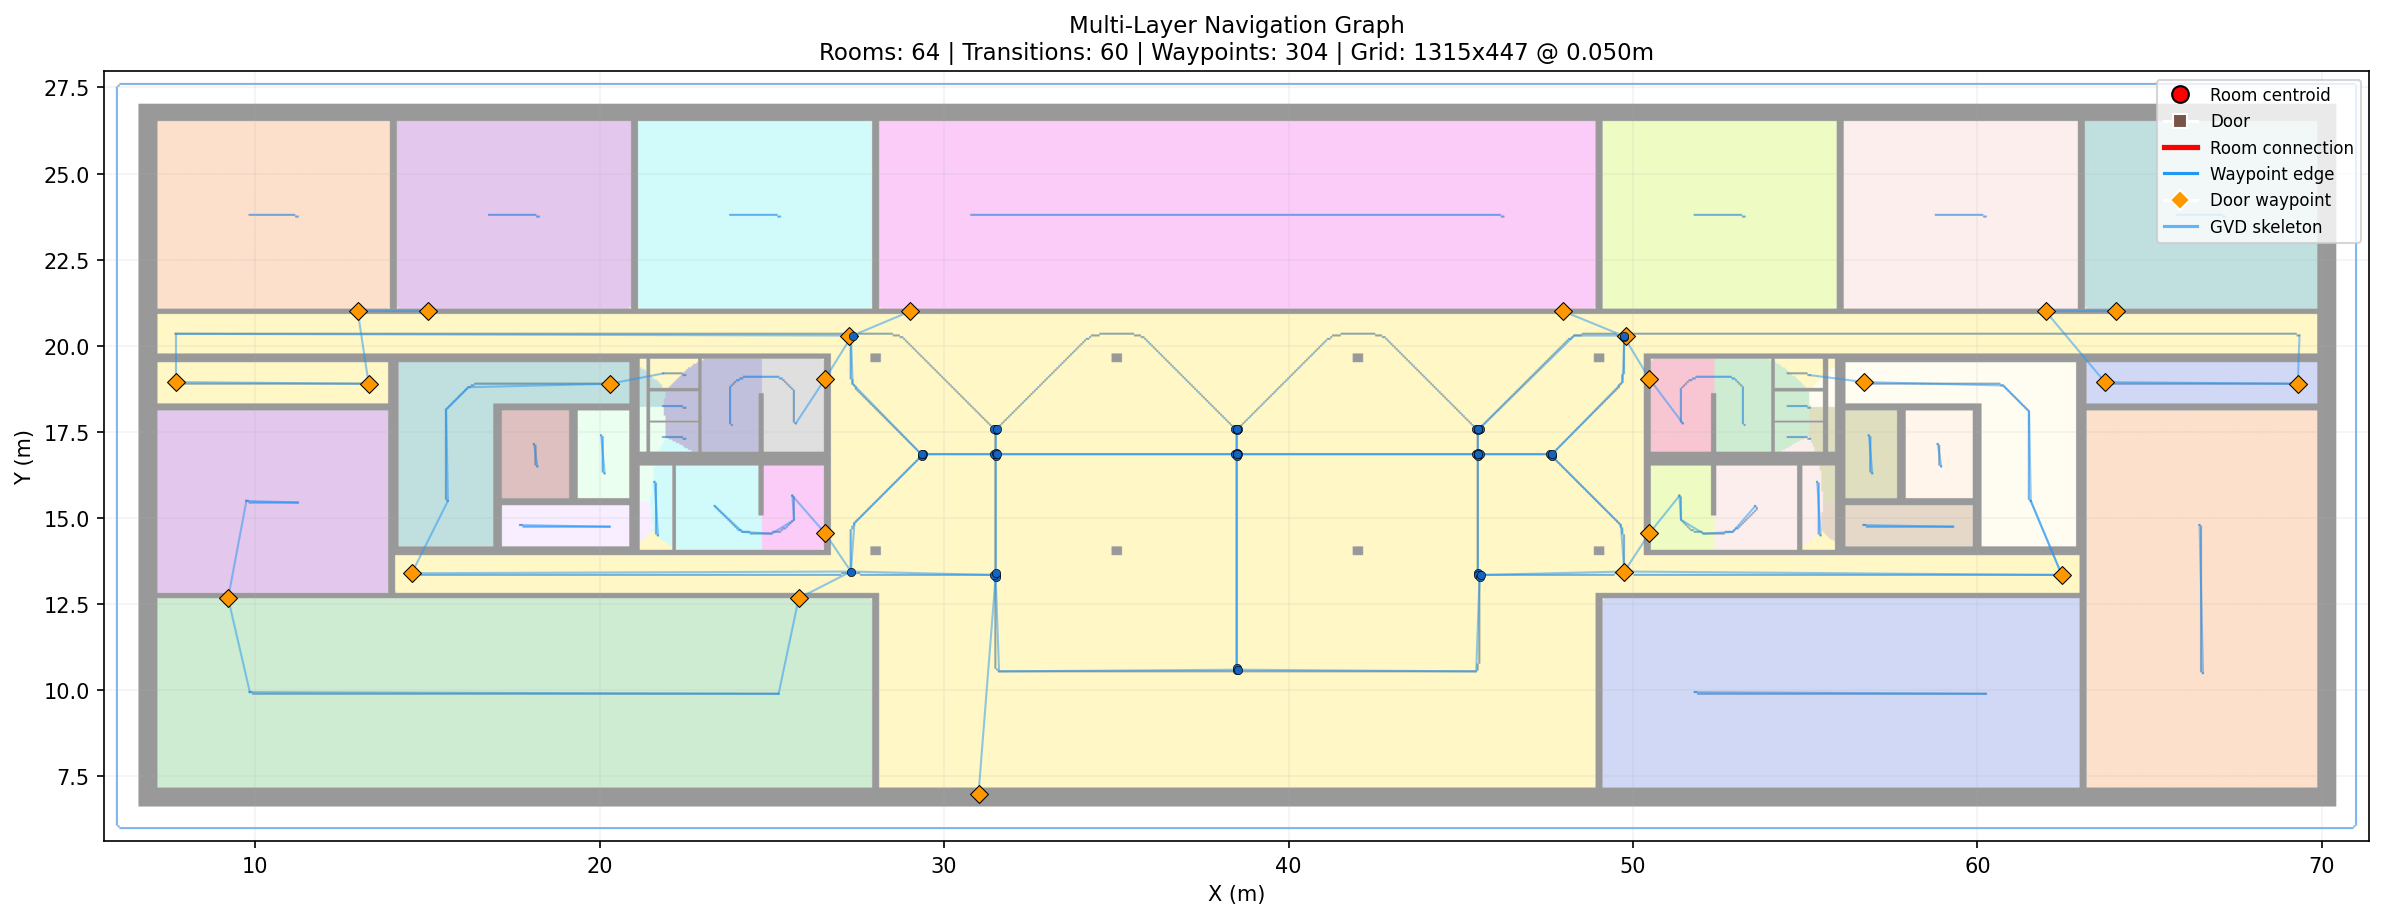
\includegraphics[width=0.95\linewidth]{figures/fig_dh_ground.png}
  \caption{Ground floor (E00\_OKRD).}
\end{subfigure}\vspace{2pt}
\begin{subfigure}[b]{\columnwidth}
  \centering
  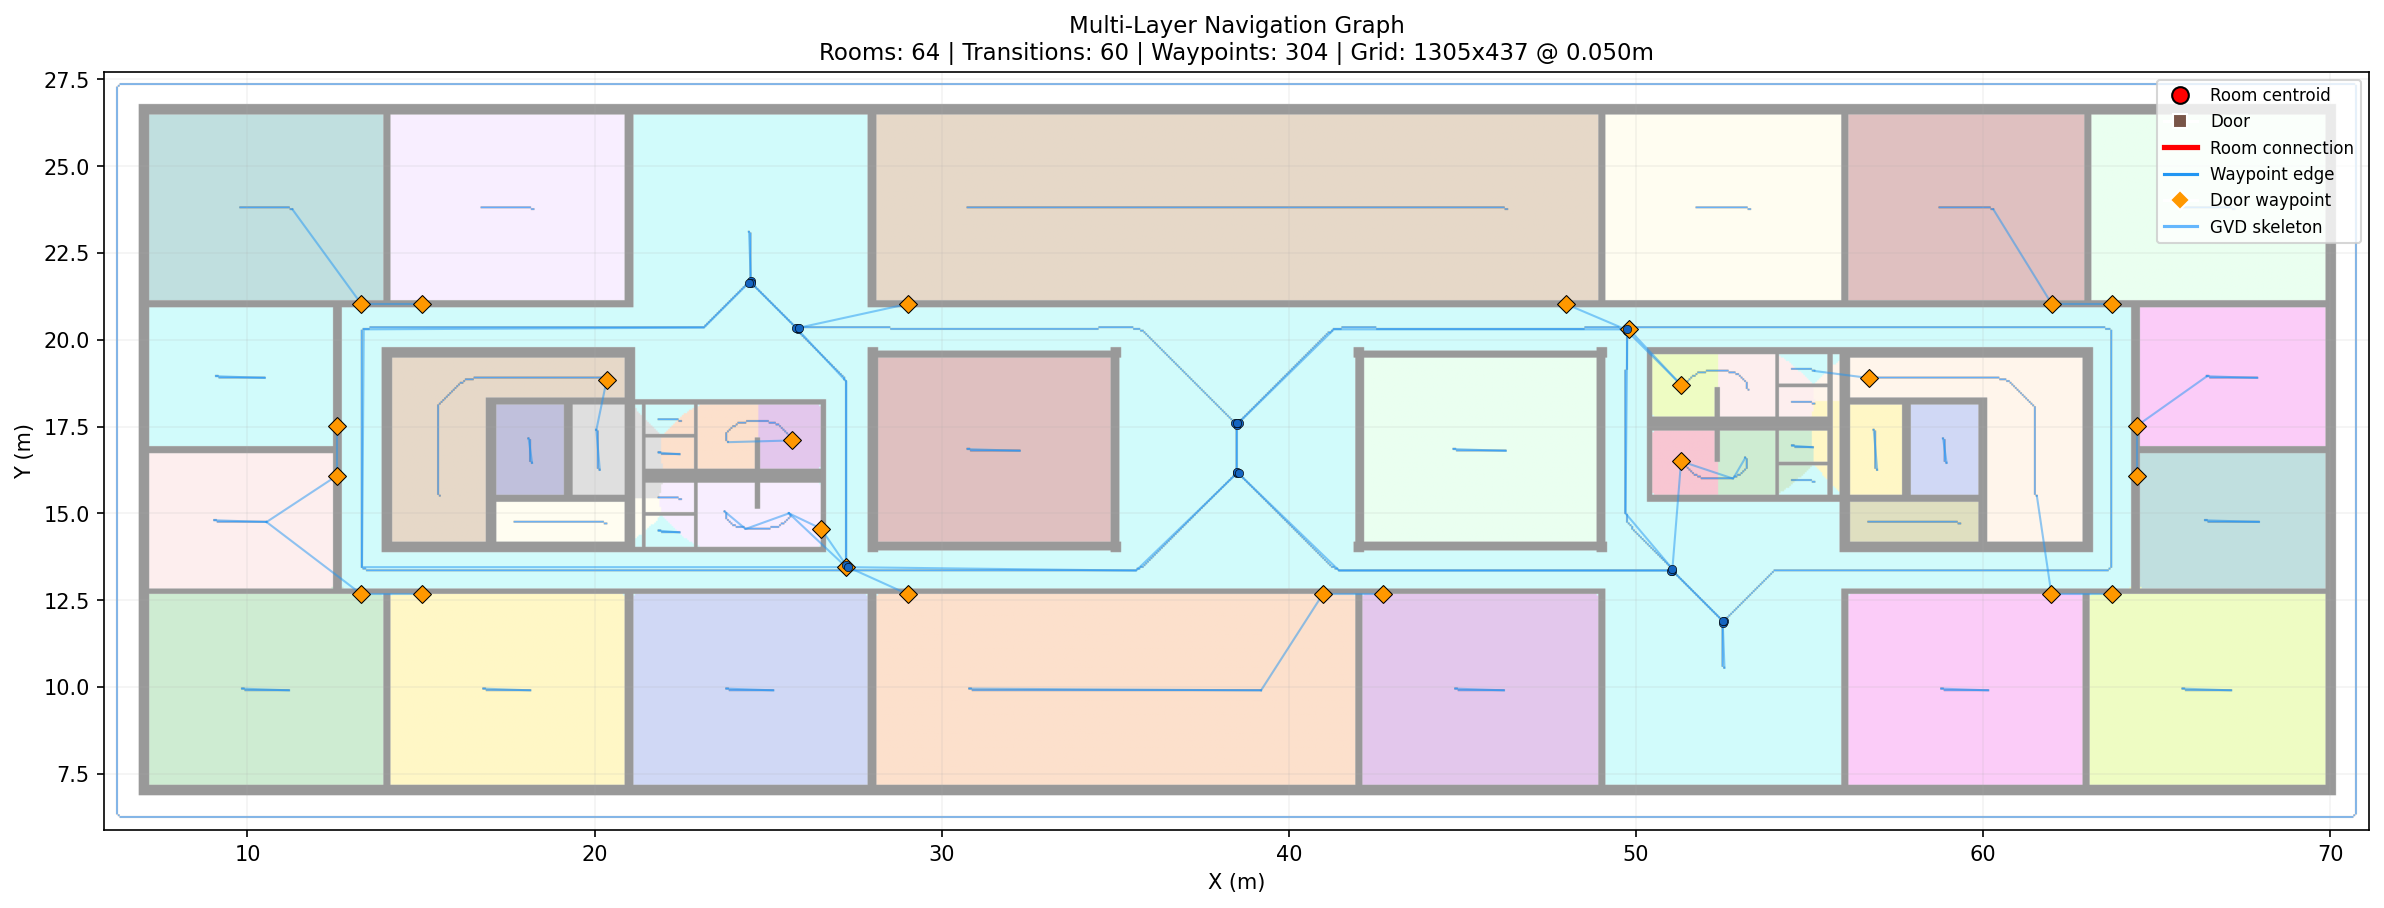
\includegraphics[width=0.95\linewidth]{figures/fig_dh_first.png}
  \caption{First floor (E01\_OKRD).}
\end{subfigure}
\vspace{-4pt}
\caption{Per-storey composite for \texttt{digital\_hub}. Each panel overlays the occupancy grid (grey), the waypoint graph (blue nodes and edges), and the room segmentation (coloured regions) on one storey of the building.}
\label{fig:dh_storeys}
\end{figure}

Fig.~\ref{fig:macalister_storeys} shows two of the six storeys in \texttt{samuel\_macalister\_sample\_house}. The dwelling has a residential layout that varies across floors, and the waypoint graph contracts around the stair and landing regions on each level.

\begin{figure}[htb]
\centering
\begin{subfigure}[b]{0.49\columnwidth}
  \centering
  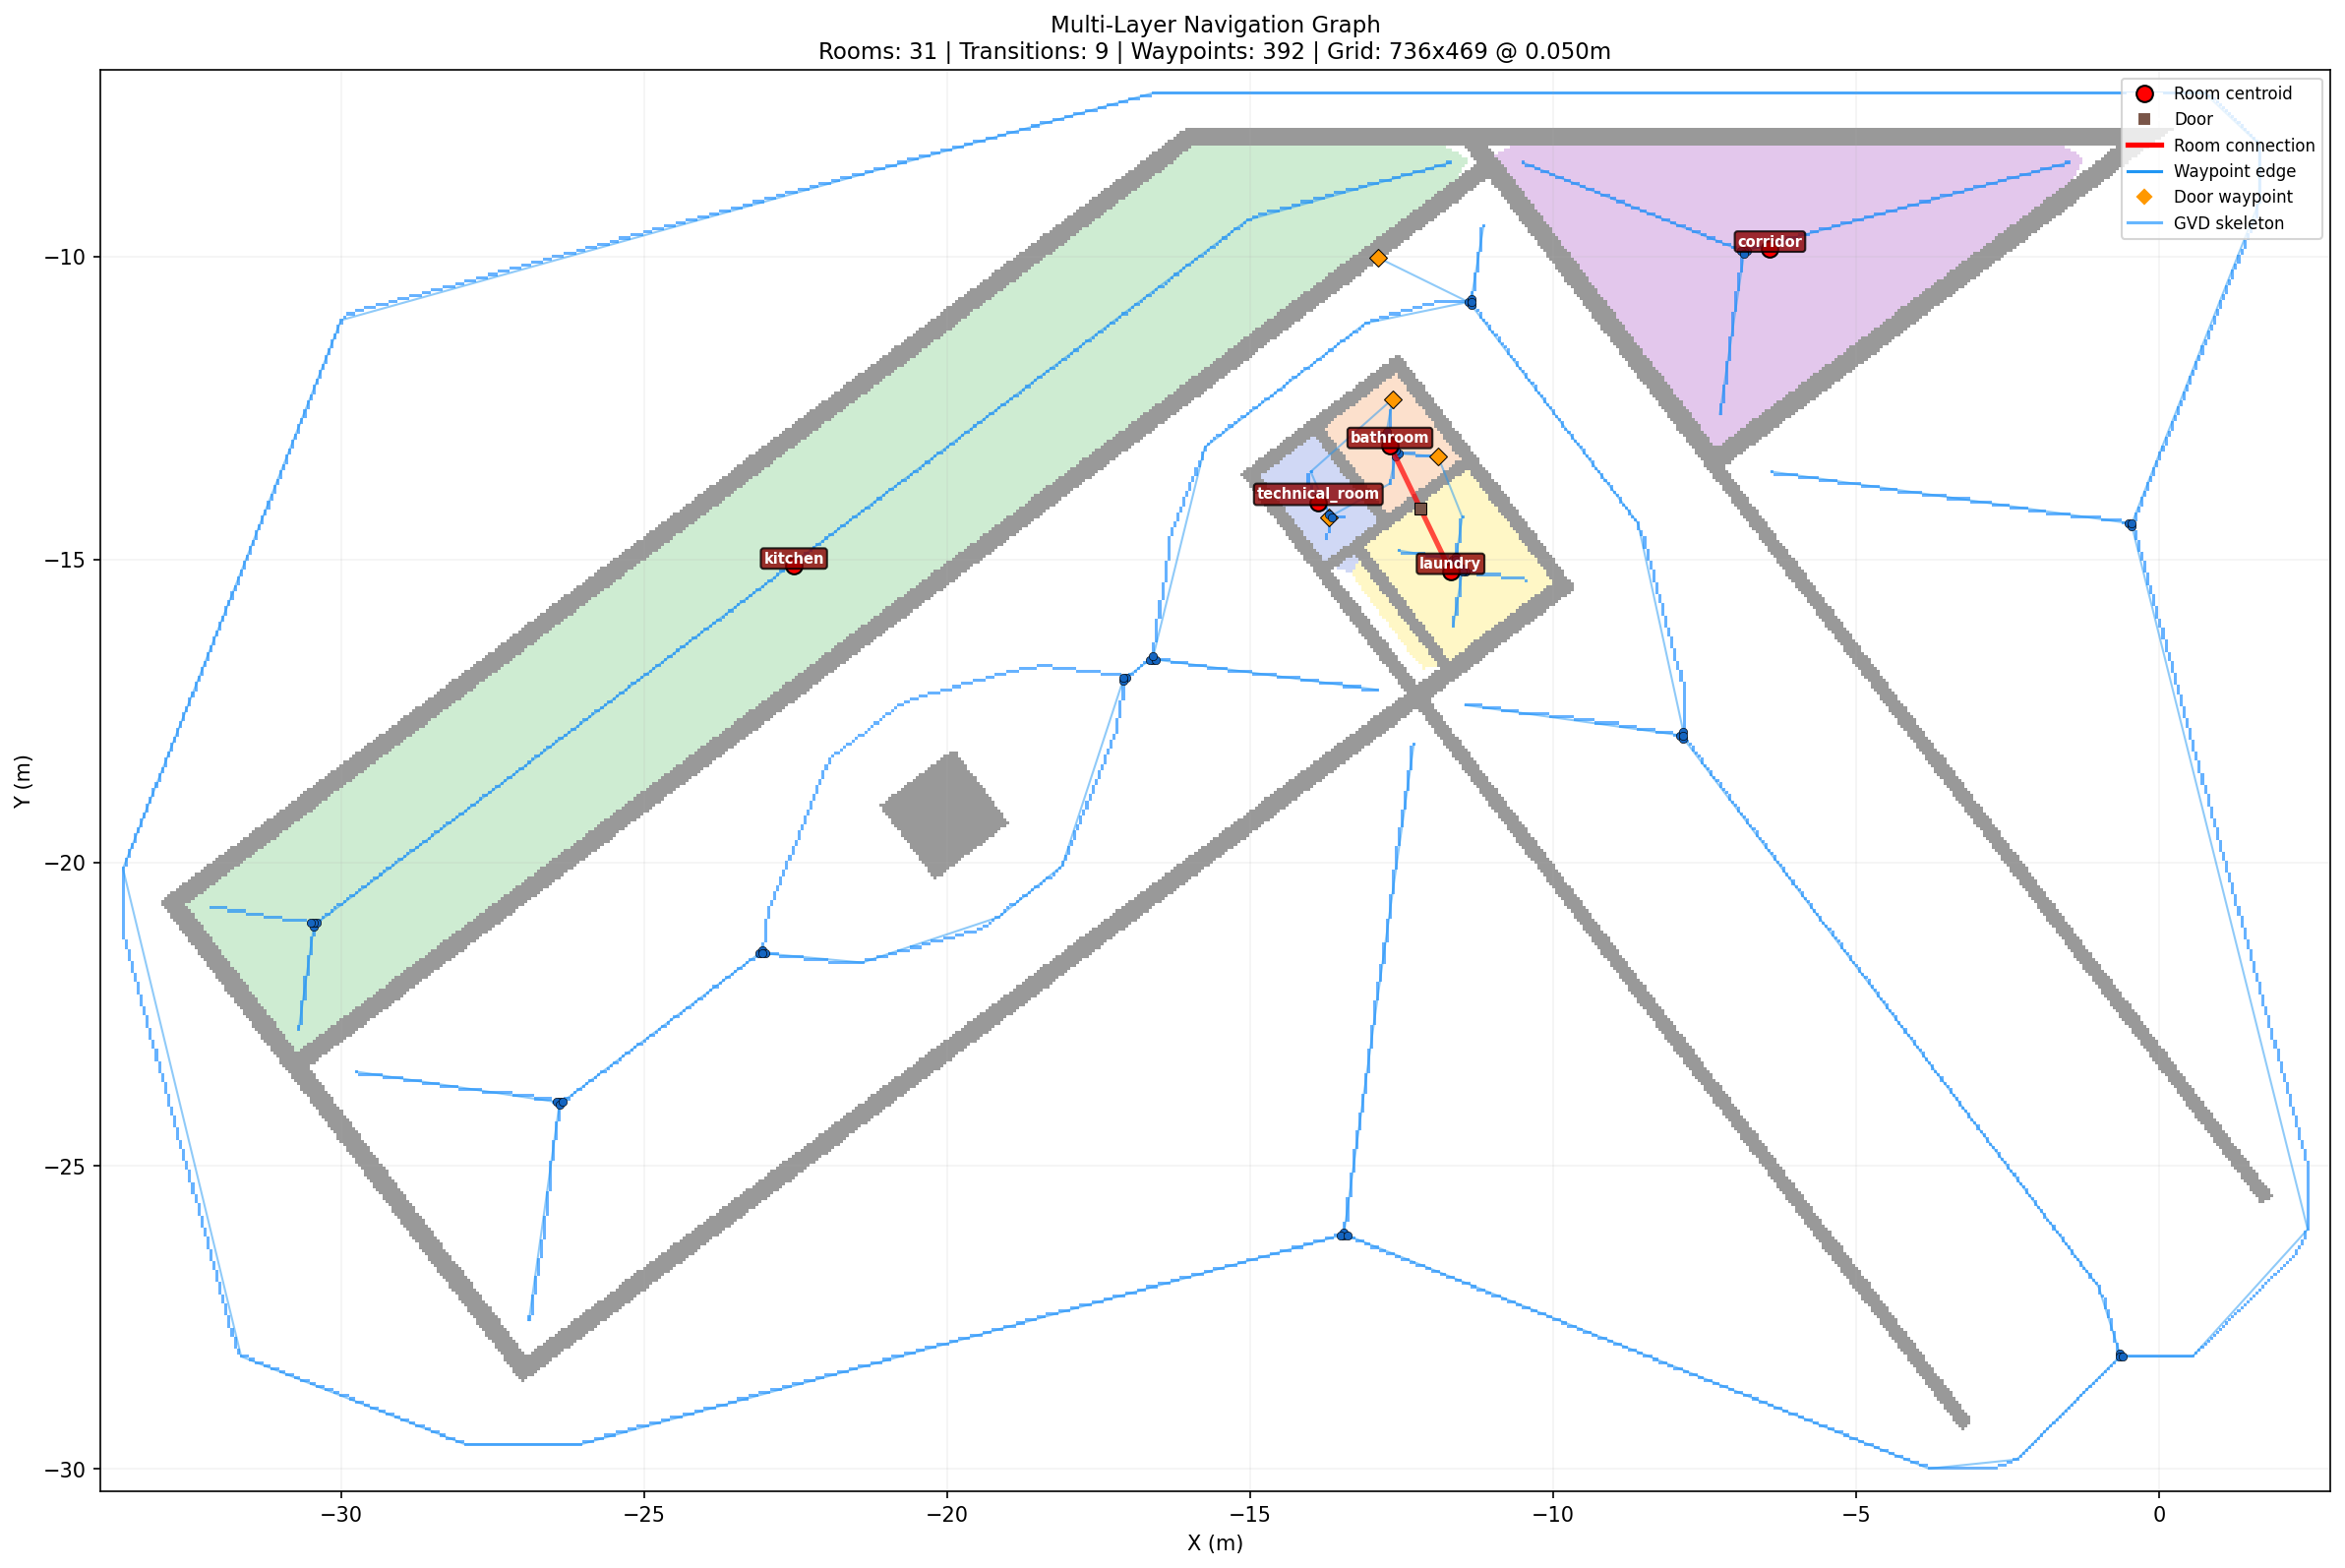
\includegraphics[width=\linewidth]{figures/fig_mac_l1.png}
  \caption{Level~1.}
\end{subfigure}\hfill
\begin{subfigure}[b]{0.49\columnwidth}
  \centering
  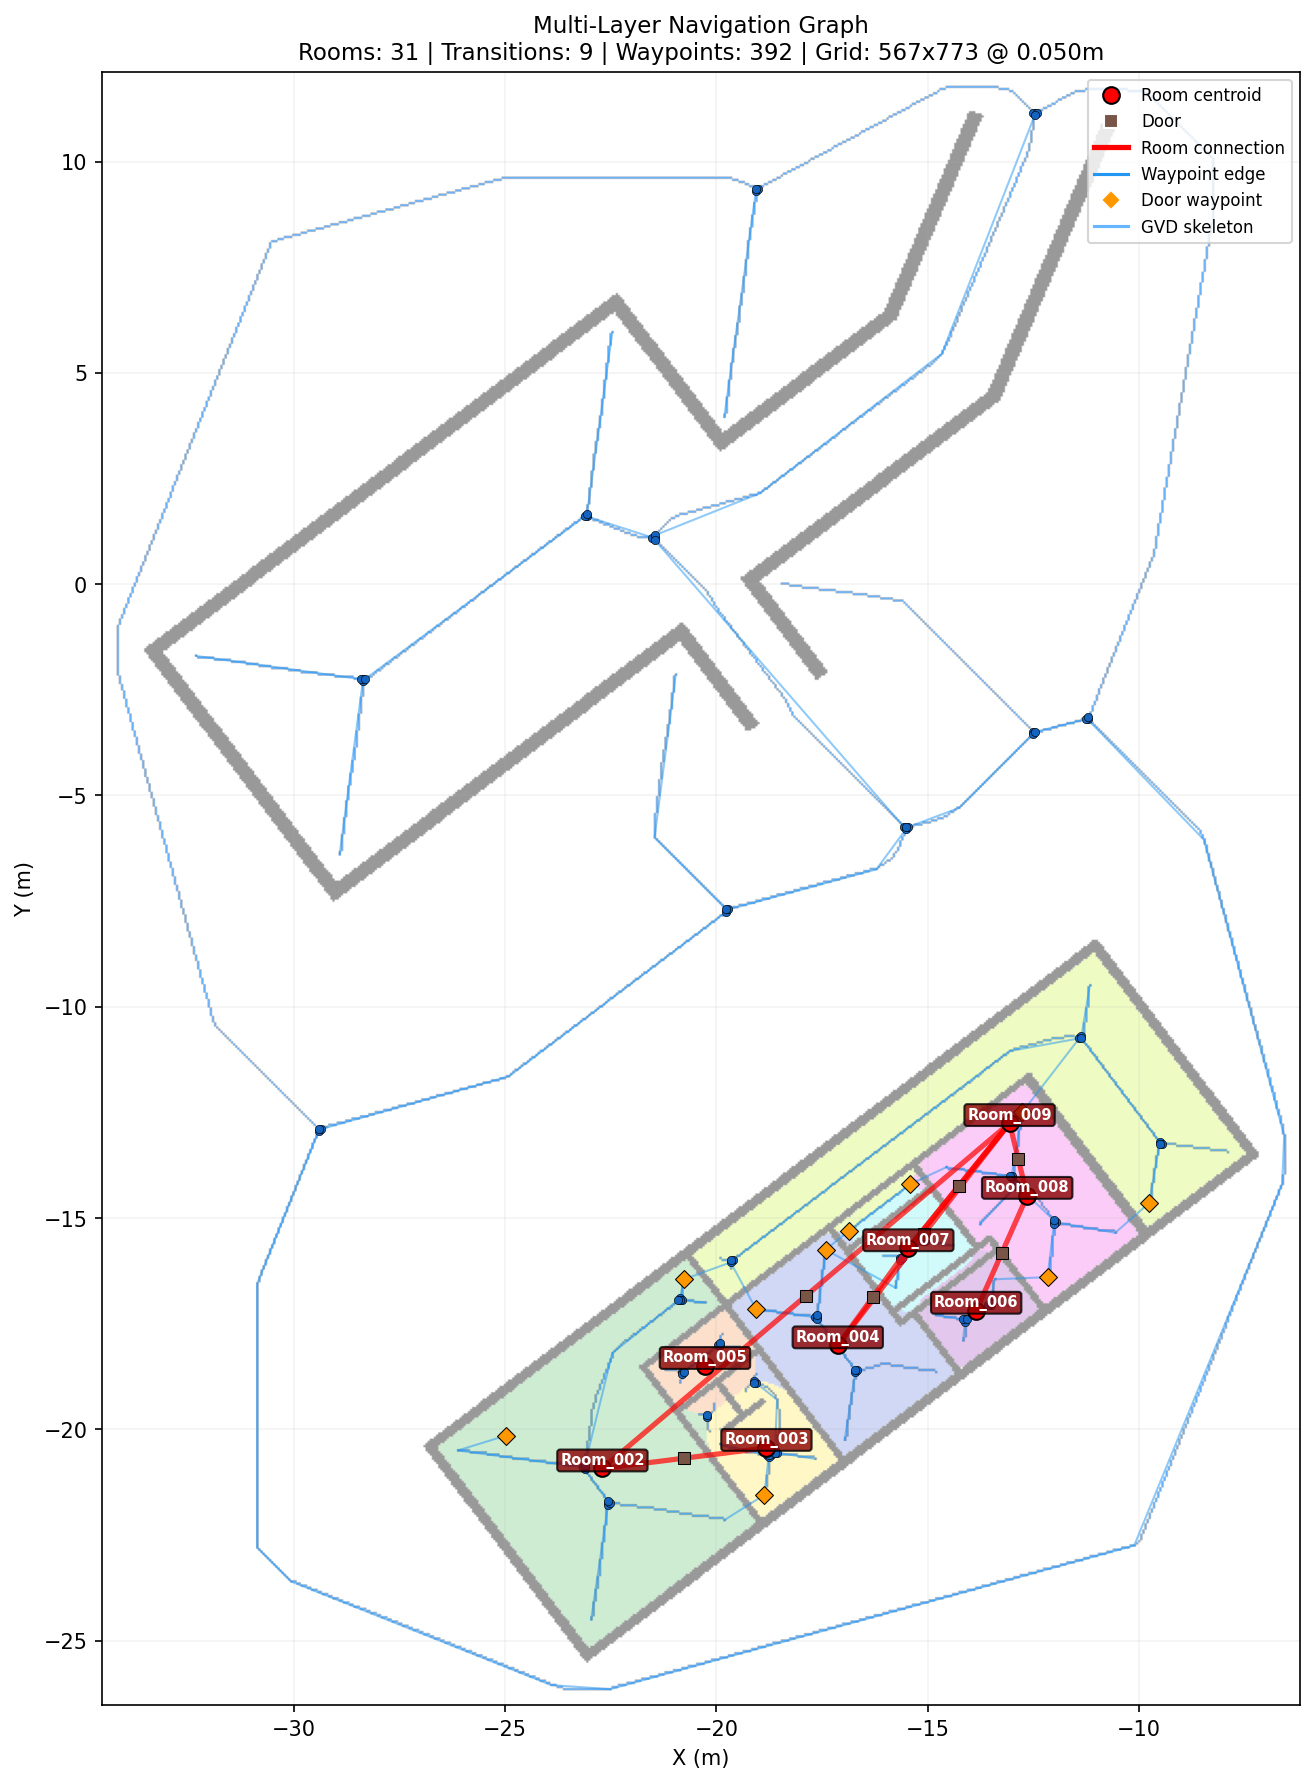
\includegraphics[width=\linewidth]{figures/fig_mac_l2.png}
  \caption{Level~2.}
\end{subfigure}
\vspace{-4pt}
\caption{Composite view on two storeys of \texttt{samuel\_macalister\_sample\_house}. The pipeline produces a consistent waypoint graph across levels, with room boundaries drawn from the authored room partitions where available.}
\label{fig:macalister_storeys}
\end{figure}

\begin{lstlisting}[caption={Short summary of the BasicHouse briefing derived from the agent trace. The full agent trace is larger and includes stage-by-stage details.},label={lst:brief},float=t!,floatplacement=t]
Room_003: living_room, concrete, trav=0.80
  hazards: [high_traffic, wet_area]
  notes:   circulation hub, 8 door transitions

Room_005: laundry, concrete, trav=0.50
  hazards: [wet_area, obstacle_dense]
  notes:   narrow channels around appliances

Room_007: bathroom, concrete, trav=0.60
  hazards: [wet_area]
  notes:   constrained layout, plumbing fixtures

Room_008: storage, concrete, trav=0.90
  hazards: [narrow_passage]
  notes:   small walk-in closet

derived_policies:
  tightest_door_m:       0.91
  width_limit_m:         0.81
  caution_rooms:         [Room_003, Room_005, Room_007]
  non_navigable_storeys: [Floor_1]
\end{lstlisting}

\end{document}
